\documentclass{article}

\usepackage{microtype}
\usepackage{graphicx}
\usepackage{subcaption}
\usepackage{booktabs}
\usepackage{hyperref}
\usepackage{amsmath}
\usepackage{amssymb}
\usepackage{mathtools}
\usepackage{url}
\usepackage{multirow}
\usepackage{xcolor}
\usepackage{siunitx}
\usepackage[round]{natbib}
\sisetup{detect-weight=true,detect-family=true}

% 공식 ICML 스타일이 있으면 그것을, 없으면 동봉한 재현본을 쓴다.
\IfFileExists{icml2025.sty}{\usepackage{icml2025}}{\usepackage{icmlstub}}

\icmltitlerunning{When Detection Metrics Cannot Discriminate}

\begin{document}

\twocolumn[
\icmltitle{When Detection Metrics Cannot Discriminate:\\
Acquisition Structure and Measurement-Shift Robustness\\
in Industrial Anomaly Detection}

\begin{icmlauthorlist}
\icmlauthor{Anonymous Authors}{anon}
\end{icmlauthorlist}

\icmlaffiliation{anon}{Anonymous Institution}
\icmlkeywords{anomaly detection, time series, benchmarking, predictive maintenance,
conformal prediction, distribution shift}

\vskip 0.2in
]

\printAffiliationsAndNotice{\textit{Paper under double-blind review. Do not distribute.}}

\begin{abstract}
Public predictive-maintenance benchmarks are increasingly used to justify deep
sequence models over classical statistical monitors. We audit one such
benchmark---a hydraulic-pump vibration and current dataset distributed with an
official LSTM-Autoencoder reference analysis---and find that its headline
comparison is not supported by the data. Three results drive this conclusion.
First, the acquisition is \emph{burst-sampled}: the nominally \SI{10}{\hertz}
record consists of 599 bursts of at most 50 samples (\SI{4.9}{\second}), so the
reference pipeline's 120-sample analysis span does not fit inside \emph{any}
burst, and its stated ``\SI{10}{\second}-ahead'' horizon is unrealizable.
Second, under a leakage-controlled protocol every model we test---including a
one-line range rule---attains recall $1.000$ and average precision that rounds
to $1.000$, so detection metrics carry \emph{almost no} discriminative power
on this benchmark; the
published LSTM-AE score of $F_1=0.748$---which we reproduce to within seed
noise at $0.743$---is below what a rule with no learned parameters attains
($F_1=0.973$), and the same network reaches $0.959$ once placed inside a
leakage-controlled protocol, so the published gap measures evaluation
procedure rather than model capacity. Third, models that are indistinguishable on detection
differ by more than $5\times$ in robustness to benign measurement shift: a
pure DC offset applied to \emph{normal} data raises the false-alarm rate by
$89.7$ points for a Mahalanobis monitor but only $17.0$ points for PCA-MSPC.
Fourth, a cross-validated false-alarm rate does not describe the system that
is actually deployed: on the identical held-out block, five-fold CV reports
$0.27\%$ while the frozen configuration produces $8.23\%$, a $30\times$ gap
caused solely by which block supplies the conformal calibration set. We argue
that on benchmarks where normal and fault records are separable for trivial
reasons---here a single fault event recorded on a different day---model
selection must be driven by false-alarm behaviour under shift and by
calibration quality, not by detection scores, and that the frozen
configuration's own held-out error must be reported alongside any
cross-validated average. We release a protocol
(gap-aware windowing, burst-blocked normal-only cross-validation, conformal
calibration, and shift-perturbation gates) that makes this selection explicit
and reproducible in one command.
\end{abstract}

\section{Introduction}
\label{sec:intro}

Industrial predictive maintenance is an attractive application for deep
sequence models: data are multivariate, temporal, and abundant, while labelled
failures are rare. The standard recipe trains a reconstruction model on
normal operation and thresholds reconstruction error
\citep{malhotra2016lstmae,audibert2020usad}. Public datasets packaged with a
reference implementation have become a common entry point for practitioners,
and the reference numbers in those packages are frequently taken as the
baseline to beat.

This paper is an audit of one such package. The dataset records vibration and
current from the hydraulic pump of a fine-blanking press, and ships with a
guidebook implementing an LSTM-Autoencoder that reports
$\mathrm{Accuracy}=97.51\%$ and $F_1=0.748$ \citep{kamp2022press}. We set out
to compare classical statistical monitors against this baseline under a common
protocol. We did not obtain a comparison, because the benchmark does not
support one. What we obtained instead is a case study in how acquisition
artefacts and dataset construction can make a detection benchmark
uninformative while still producing respectable-looking numbers.

Our contributions are as follows.

\textbf{(1) The acquisition is not a continuous stream.} We show
(\S\ref{sec:data}) that the record is burst-sampled: 599 bursts whose longest
is 50 samples. The reference pipeline builds 20-sample windows with a
100-step label offset, a 120-sample span that fits inside no burst. Its
windows therefore straddle gaps of arbitrary length, and the ``10\,s ahead''
interpretation of the offset is an artefact of treating the row index as
uniform time.

\textbf{(2) Detection metrics cannot discriminate models here.} Under a
leakage-controlled protocol (\S\ref{sec:protocol}), a one-line normal-range
rule, a shrinkage Mahalanobis monitor, and PCA-MSPC all reach recall $1.000$
with AUROC above $0.9998$ (\S\ref{sec:sep}). Shape features alone give
$\mathrm{AP} = 0.9986$ and amplitude features alone $0.9935$, so the signal is
redundant across feature groups. Reporting $F_1$ differences on this benchmark
measures threshold placement, not detection ability.

\textbf{(3) Robustness to benign measurement shift does discriminate, by a
wide margin.} Perturbing \emph{normal} data with sensor gain, DC offset,
polarity inversion and sampling jitter---changes that a maintenance system
must not report as equipment faults---separates the models cleanly
(\S\ref{sec:robust}): worst-case false-alarm increase ranges from $17.0$ to
$89.7$ percentage points. We make this the selection criterion.

\textbf{(4) The protocol choices are load-bearing, and we measure by how much.}
Against a uniform random score the submitted detector is clearly separated
($F_1$ $0.994$ vs.\ $0.228$), but under the point-adjustment protocol that is
standard in much of this literature a \emph{random} score reaches $F_1=0.779$
--- indistinguishable from our deployed system's operational $0.780$
(\S\ref{sec:protoval}). Reporting against a trivial baseline and refusing
point adjustment are therefore not stylistic preferences here; either omission
would have reversed the paper's conclusion.

\textbf{(5) A reproducible protocol.} We specify gap-aware windowing,
burst-blocked normal-only block cross-validation, split-conformal calibration
of the alarm threshold, and a sequence of selection gates that deliberately
excludes detection score as a tie-breaker (\S\ref{sec:protocol}). The full
pipeline runs end-to-end in \SI{25}{\second} on a laptop CPU.

We state plainly what this benchmark cannot support. The fault class is a
single continuous recording made five days after the normal recording, so
perfect separability is confounded with date, operating condition and sensor
state; and because the fault record begins after the equipment state has
already changed, no lead-time claim is measurable. We treat these as
properties of the benchmark to be reported, not obstacles to be modelled
around.

\section{Related Work}
\label{sec:related}

\paragraph{Evaluation pathologies in time-series anomaly detection.}
A growing literature argues that progress in this area is partly illusory.
\citet{kim2022towards} show that the widely used \emph{point-adjustment}
protocol inflates $F_1$ so severely that random scores appear
state-of-the-art, and \citet{wu2023current} argue that several standard
benchmarks are trivially solvable or mislabelled. \citet{garg2022evaluation}
reach similar conclusions in a systematic comparison. Our finding is adjacent
but distinct: we do not use point adjustment, and the failure is not
mislabelling. The benchmark is simply \emph{too separable}, so every method
saturates and the metric stops ordering methods. We therefore argue for
replacing the ordering criterion rather than only repairing the metric.

\paragraph{Shortcut learning and confounded splits.} That a model may key on a
nuisance correlate rather than the phenomenon of interest is well documented
in vision and medical imaging \citep{geirhos2020shortcut,zech2018variable},
where scanner or site identity can be predicted more easily than pathology;
\citet{recht2019imagenet} show how fragile benchmark conclusions can be to
distribution details. The present dataset has the same structure in a
particularly stark form: class is perfectly aligned with acquisition date.

\paragraph{Classical multivariate process monitoring.} Hotelling's $T^2$ with
squared prediction error (SPE/$Q$) is the standard tool for industrial
monitoring \citep{jackson1979control,qin2003statistical}, and provides
per-variable contribution plots that support root-cause triage. We use it,
shrinkage covariance estimation \citep{ledoit2004well}, and Isolation Forest
\citep{liu2008isolation} as the comparison set against the reference
LSTM-Autoencoder.

\paragraph{Distribution-free calibration.} We set alarm thresholds by
split-conformal $p$-values \citep{vovk2005algorithmic,angelopoulos2023conformal},
which give a distribution-free statement about normal operation without ever
consulting fault labels. Because overlapping windows violate exchangeability,
we block by acquisition burst, in the spirit of purged cross-validation
\citep{lopezdeprado2018advances}, and we report realized coverage rather than
assuming it.

\section{Problem Formulation}
\label{sec:prelim}

We first fix notation. Our departure from the standard time-series anomaly
detection (TAD) setup is confined to \S\ref{sub:bursts}, where the acquisition
is not a uniformly sampled stream; everything downstream inherits that change.

\subsection{Signals and labels}

Let $X=(x_1,\dots,x_T)$ denote a record of $N$ synchronous channels, $x_t\in
\mathbb{R}^{N}$, observed at timestamps $\tau_1<\dots<\tau_T$. Here $N=3$
(upper vibration, lower vibration, motor current). Write
$\Delta_t=\tau_{t+1}-\tau_t$ for the sampling interval. A binary label
$y_t\in\{0,1\}$ marks fault ($1$) or normal ($0$).

Two properties of this benchmark are atypical and must be carried in the
notation. First, $y_t$ is constant within each record: the label is a property
of the \emph{file}, not of the sample. Second, the normal and fault records
were acquired on different days; writing $c(t)\in\{1,2\}$ for the acquisition
session of sample $t$, we have $y_t=\mathbb{1}[c(t)=2]$ exactly. Session and
label are perfectly confounded, which is the premise of \S\ref{sec:robust}.

\subsection{Acquisition bursts}
\label{sub:bursts}

The standard setup assumes $\Delta_t$ constant. It is not. Fix a gap threshold
$g$ and define the \emph{acquisition bursts} as the maximal contiguous runs
\begin{equation}
\mathcal{B}=\{B_1,\dots,B_K\},\qquad
B_k=\{t: a_k \le t \le b_k\},\ \ \Delta_t\le g\ \ \forall\, t\in[a_k,b_k),
\label{eq:burst}
\end{equation}
so that consecutive bursts are separated by $\Delta_{b_k}>g$. We use
$g=\SI{0.5}{\second}$. A burst is the natural unit of this acquisition: it is
the longest stretch over which "adjacent sample" means what it usually means.

\subsection{Gap-aware windowing}

Given a window length $\ell$, the naive stride-1 construction is
$w_t=(x_t,\dots,x_{t+\ell-1})$ for every admissible $t$. We instead require a
window to lie entirely inside one burst,
\begin{equation}
\mathcal{W}_\ell=\bigl\{\,w_t \;:\; [t,\,t+\ell-1]\subseteq B_k \text{ for some } k \,\bigr\},
\label{eq:gapaware}
\end{equation}
and define the \emph{survival rate}
$\rho(\ell)=|\mathcal{W}_\ell| \,/\, |\mathcal{W}^{\mathrm{naive}}_\ell|$,
the fraction of naive windows that are physically contiguous. A window outside
$\mathcal{W}_\ell$ concatenates signal segments separated by up to
\SI{16.6}{\second} and therefore contains a discontinuity of instrumental, not
mechanical, origin. Section~\ref{sec:data} measures $\rho$.

A feature map $\phi:\mathbb{R}^{\ell\times N}\!\to\mathbb{R}^{d}$ summarises
each window; $d=23$ here, grouped as amplitude, shape, relation and level
(\S\ref{sec:protocol}).

\subsection{Scoring and decision}

A detector is a score $A:\mathbb{R}^{d}\!\to\mathbb{R}$, larger meaning more
anomalous, fitted on normal data only. Rather than thresholding $A$ directly we
convert it to a split-conformal $p$-value against a normal calibration set
(Eq.~\ref{eq:conformal}) and alarm when
\begin{equation}
\hat y_t=\mathbb{1}\!\left[\,p_{\mathrm{normal}}(\phi(w_t))\le\alpha\,\right],
\qquad \alpha=0.01 .
\label{eq:decide}
\end{equation}
We write $\mathrm{risk}=1-p_{\mathrm{normal}}$ and stress that it is a rank
statistic, not $\Pr(y=1\mid x)$; \S\ref{sec:calib} measures the gap.

\subsection{Temporal integration}

Single-window decisions are debounced. For integers $M\le N_{\mathrm w}$ define
the operator
\begin{equation}
\Pi_{N_{\mathrm w},M}(\hat y)_t=\mathbb{1}\!\left[\textstyle\sum_{j=t-N_{\mathrm w}+1}^{t}\hat y_j\ \ge M\right],
\label{eq:mofn}
\end{equation}
evaluated only over index windows contained in a single burst. The submitted
system uses the strict form $N_{\mathrm w}=M=3$. Section~\ref{sec:mofn}
measures the whole $(N_{\mathrm w},M)$ family; the usual recommendation that
loose integration ($M<N_{\mathrm w}$) helps turns out to be false here.

\subsection{Three evaluation levels}
\label{sub:levels}

Results are reported at three granularities, and mixing them silently is the
error this paper is most concerned with.

\begin{description}\itemsep2pt
\item[$\mathcal{L}_1$ window.] Each $w\in\mathcal{W}_\ell$ is one observation.
  Overlapping windows share $\ell-1$ of $\ell$ samples, so these are not
  independent.
\item[$\mathcal{L}_2$ burst.] Each $B_k$ is one observation; a burst is called
  detected if any of its windows alarms. This is the smallest plausibly
  exchangeable unit, and all confidence intervals resample at this level.
\item[$\mathcal{L}_3$ event.] A maximal run of alarming windows is one alarm
  event; false-alarm rates per hour are counted here.
\end{description}

With $P,R,F_1$ defined as usual from $\mathrm{TP},\mathrm{FP},\mathrm{FN}$, the
\emph{effective} number of positive observations is not $|\{t:y_t=1\}|$ but the
number of independent fault events, which is \textbf{one}. Any interval
estimate that ignores this is meaningless, so we resample bursts rather than
windows throughout.

\subsection{Point adjustment, and why we do not use it}
\label{sub:pa}

Let $\mathcal{S}=\{S_1,\dots,S_M\}$ be the ground-truth fault segments. The
widely used \emph{point-adjustment} (PA) protocol \citep{kim2022towards}
replaces $\hat y$ by
\begin{equation}
\hat y^{\mathrm{PA}}_t=
\begin{cases}
1, & t\in S_m \text{ and } \exists\, t'\!\in S_m:\ \hat y_{t'}=1,\\
\hat y_t, & \text{otherwise,}
\end{cases}
\label{eq:pa}
\end{equation}
that is, one hit anywhere inside a segment credits the whole segment. PA can
only increase $\mathrm{TP}$ and decrease $\mathrm{FN}$, never touching
$\mathrm{FP}$, so $F_1^{\mathrm{PA}}\ge F_1$ always. We take $S_m$ to be the
fault bursts. \textbf{We report no adjusted metric anywhere in this paper};
\S\ref{sec:protoval} measures what PA would have done to our numbers, and the
answer is the reason for the choice.

\section{The Benchmark and Its Acquisition Structure}
\label{sec:data}

\paragraph{Dataset.} The package \citep{kamp2022press} contains two CSV files
from a fine-blanking press hydraulic pump: a normal record of $20{,}000$ rows
(2022-07-12) and a fault record of $600$ rows (2022-07-17). Each row carries
upper and lower pump vibration (\texttt{AI0}, \texttt{AI1}), motor current
(\texttt{AI2}), and a constant equipment-state flag---$0$ throughout the
normal file and $1$ throughout the fault file. Sampling is documented as
10 times per second.

\paragraph{The record is burst-sampled.} Table~\ref{tab:e0} reports the
audit. The normal file spans \SI{4615.8}{\second} of wall-clock time while
containing only \SI{2000}{\second} worth of samples at \SI{10}{\hertz}; 598
inter-sample gaps exceed \SI{0.5}{\second}. Segmenting at those gaps yields
599 bursts with median 37 and maximum 50 samples---at most
\SI{4.9}{\second} of contiguous signal. The fault file is identical in
character: 21 bursts, maximum 50 samples. Figure~\ref{fig:burst} visualises
the structure.

\begin{table}[t]
\caption{Acquisition audit. ``Span if continuous'' is the duration the row
count would occupy at the documented \SI{10}{\hertz}. The discrepancy is the
total gap time.}
\label{tab:e0}
\vskip 0.08in
\centering
\small
\begin{tabular}{lrr}
\toprule
 & Normal & Fault \\
\midrule
Rows                         & 20{,}000 & 600 \\
Observed span (s)            & 4615.8   & 165.6 \\
Span if continuous (s)       & 2000.0   & 60.0 \\
Median $\Delta t$ (s)        & 0.100    & 0.100 \\
Gaps $>\SI{0.5}{\second}$    & 598      & 20 \\
Bursts                       & 599      & 21 \\
Burst length (median / max)  & 37 / 50  & 28 / 50 \\
Bursts $\ge 120$ samples     & \textbf{0} & \textbf{0} \\
Missing values               & 0        & 0 \\
\bottomrule
\end{tabular}
\end{table}

\begin{figure}[t]
\centering
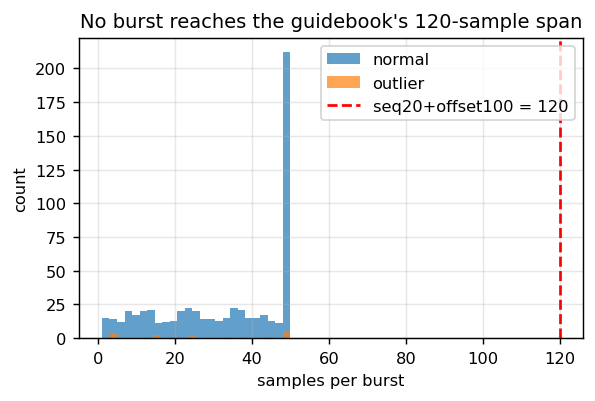
\includegraphics[width=\columnwidth]{figures/fig2_burst_length.png}
\caption{Burst length distribution. The reference pipeline's analysis span
(20-sample window $+$ 100-step offset $=$ 120 samples, dashed line) exceeds
every burst in both files.}
\label{fig:burst}
\end{figure}

\paragraph{Consequence for the reference pipeline.} The guidebook builds
windows of 20 consecutive \emph{rows} and pairs them with a label 100 rows
later, describing this as detecting conditions \SI{10}{\second} ahead. Because
no burst reaches 120 samples, that span always crosses at least one gap, and
the realized time offset is not \SI{10}{\second} but an uncontrolled quantity
determined by gap durations. Two consequences follow: the temporal-horizon
claim is unrealizable, and a substantial fraction of ``2-second'' windows are
not contiguous in time at all. Enforcing that windows lie inside a single
burst removes $25.6\%$ of windows at length 10 and $50.1\%$ at length 20
(Table~\ref{tab:e1}); those removed windows are precisely the fictitious ones.

\begin{table}[t]
\caption{Windows retained when windows are confined to a single burst,
relative to naive index-contiguous windowing.}
\label{tab:e1}
\vskip 0.08in
\centering
\small
\begin{tabular}{crrrr}
\toprule
\multirow{2}{*}{Length} & \multicolumn{2}{c}{Normal} & \multicolumn{2}{c}{Fault} \\
\cmidrule(lr){2-3}\cmidrule(lr){4-5}
 & Gap-aware & Retained & Gap-aware & Retained \\
\midrule
5  & 17{,}652 & 88.3\% & 517 & 86.7\% \\
10 & 14{,}871 & 74.4\% & 428 & 72.4\% \\
20 & \phantom{0}9{,}978 & 49.9\% & 276 & 47.5\% \\
\bottomrule
\end{tabular}
\end{table}

\paragraph{What the labels mean.} The fault file is a single uninterrupted
recording of an \emph{already faulted} machine; the equipment-state flag is
constant within each file. The 428 fault windows at length 10 are therefore
overlapping fragments of \emph{one} event, not 428 independent positives, and
no pre-failure segment exists. We report window counts for transparency but
treat the number of independent positive events as one throughout.

\section{Protocol}
\label{sec:protocol}

We fix the following before examining any result; deviations made after seeing
results are logged explicitly (\S\ref{sec:amend}).

\paragraph{Windowing.} Windows are 10 samples with stride 1 and must lie
entirely within one burst. Window length 5 and 20 are reported as sensitivity.

\paragraph{Features.} From each window we compute four interpretable groups:
\textbf{A} amplitude (per-channel standard deviation, peak-to-peak, RMS),
\textbf{S} shape (lag-1 and lag-2 autocorrelation, zero-crossing rate),
\textbf{R} relation (\texttt{AI0}--\texttt{AI1} correlation, absolute-value
correlation, standard-deviation ratio), and \textbf{O} level (current mean and
mean absolute value). A fifth group \textbf{Q} (sampling-interval variability,
position within burst) is computed for diagnosis but excluded from model input
so that acquisition artefacts cannot be mistaken for fault evidence. This
yields a 23-dimensional model input.

\paragraph{Block cross-validation on normal data only.} The normal record is
partitioned into five contiguous blocks \emph{by burst}, so no burst is split
across blocks. Each fold uses three blocks for fitting, one for calibration,
and one as normal hold-out, rotating so each block is hold-out exactly once.
Random $k$-fold and window-level shuffling are prohibited: overlapping windows
would place near-duplicates on both sides of the split.

\paragraph{Conformal alarm threshold.} All scalers and thresholds are fit on
the fitting and calibration blocks only. Given calibration scores
$s_1,\dots,s_n$ from normal data, a new window receives
\begin{equation}
p_{\text{normal}}(x) \;=\; \frac{1 + |\{i : s_i \ge s(x)\}|}{n+1},
\label{eq:conformal}
\end{equation}
and we alarm when $p_{\text{normal}} \le \alpha$ with $\alpha = 0.01$. We
define $\mathrm{risk} = 1 - p_{\text{normal}}$ and emphasise that this is a
rank statistic, not a posterior probability of failure; a prevalence
sensitivity table is reported separately. Fault data are never used to choose
thresholds, features or hyperparameters.

\paragraph{Models.} \textbf{BL-0}, a range rule flagging any feature outside
its training min--max; \textbf{M1}, shrinkage Mahalanobis distance
\citep{ledoit2004well}; \textbf{M2}, Isolation Forest \citep{liu2008isolation};
\textbf{M3}, PCA-MSPC combining $T^2$ and SPE \citep{jackson1979control}; and
\textbf{BL-1}, the reference LSTM-Autoencoder reproduced exactly
($64\!\to\!32\!\to$ repeat $\to\!32\!\to\!64$, mean-squared reconstruction
loss) in two variants defined in \S\ref{sec:bl1}.

\paragraph{Metrics.} We report window-level recall, precision, $F_1$, MCC,
average precision (AP) and AUROC; false-alarm window rate and merged alarm
events per hour on each normal hold-out block, with a Poisson 95\% upper bound
so that a zero count is never reported as a rate of zero; realized conformal
coverage; and false-alarm increase under measurement perturbation. We report
the worst block, not only the mean.

\section{Protocol Validation: A Random Baseline and Point Adjustment}
\label{sec:protoval}

Two choices in \S\ref{sec:protocol} --- reporting against a trivial baseline,
and refusing point adjustment --- are easy to assert and easy to skip. We
measure what each is worth on this benchmark. Both experiments use the normal
hold-out ($2{,}929$ windows) together with all fault windows ($428$ windows in
$17$ segments), and both report the \emph{oracle} $F_1$ obtained by sweeping the
threshold to its best value, which is the quantity most favourable to the
method under test.

\begin{table}[t]
\centering\small
\caption{Oracle $F_1$ under each protocol. Uniform random scores are averaged
over 20 seeds ($\pm$ s.d.). Our operational threshold is the conformal rule of
Eq.~\ref{eq:decide}, not an oracle sweep.}
\label{tab:protoval}
\setlength{\tabcolsep}{4pt}
\begin{tabular}{@{}llr@{}}
\toprule
Score & Prot. & $F_1$ \\
\midrule
Submitted, oracle $\delta$ & --- & 0.994 \\
Uniform random, oracle $\delta$ & --- & 0.228\,$\pm$\,0.002 \\
Submitted, conformal $\alpha{=}0.01$ & --- & 0.780 \\
\midrule
Submitted, oracle $\delta$ & PA & 1.000 \\
Uniform random, oracle $\delta$ & PA & \textbf{0.779\,$\pm$\,0.041} \\
\bottomrule
\end{tabular}
\end{table}

\paragraph{A random baseline is not free.} \citet{kim2022towards} argue that
TAD results are uninterpretable without a trivial reference, because the class
balance and segment structure of these benchmarks can carry a large $F_1$ on
their own. On our split a uniform random score reaches $F_1=0.228$ at its best
threshold (Table~\ref{tab:protoval}), well below the submitted detector's
$0.994$. The separation is therefore real --- but note the second row against
the third: our \emph{deployed} conformal threshold yields $0.780$, not $0.994$.
The gap between oracle and operational thresholding is larger than the gap
between several of the models we compare in \S\ref{sec:sep}, which is one more
reason not to rank detectors on $F_1$ here.

\paragraph{Point adjustment would have erased the comparison.} Applying
Eq.~\ref{eq:pa}, the submitted detector reaches $F_1^{\mathrm{PA}}=1.000$ and a
\emph{uniform random score} reaches $0.779\pm0.041$. The latter is
indistinguishable from the operational $F_1$ of our actual system. Had we
adopted the protocol that is standard in much of this literature, a detector
with no information would have matched a deployed one, and the entire empirical
content of this paper would have been an artefact of the metric.

\begin{table}[t]
\centering\small
\caption{PA inflation of a random score grows as fault segments get shorter.
Segments are fault bursts, ordered by length; each row keeps the shortest
$p\%$. Five seeds.}
\label{tab:painflate}
\begin{tabular}{lccccc}
\toprule
Subset & Segments & Median len. & $F_1$ & $F_1^{\mathrm{PA}}$ & Inflation \\
\midrule
shortest 25\% & 4  & 6  & 0.030 & 0.173 & $\times 5.8$ \\
shortest 50\% & 8  & 12 & 0.067 & 0.439 & $\times 6.5$ \\
all           & 17 & 27 & 0.227 & 0.788 & $\times 3.5$ \\
\bottomrule
\end{tabular}
\end{table}

\paragraph{The inflation is structural, not incidental.}
Table~\ref{tab:painflate} restricts to the shortest segments and recomputes.
Inflation is largest where segments are short, because PA converts a single
chance hit into credit for the whole segment regardless of its length; with
$17$ segments of median $27$ windows, a random score needs only one hit per
segment. This is the mechanism \citet{kim2022towards} identify, reproduced on
an industrial benchmark that their study does not cover. It also explains why
burst-level reporting (\S\ref{sub:levels}, $\mathcal{L}_2$) is \emph{not} a
disguised form of PA: $\mathcal{L}_2$ counts a burst once, whereas PA counts it
as many times as it has windows.

\section{Normal and Fault Are Perfectly Separable}
\label{sec:sep}

Table~\ref{tab:e2} gives the five-fold result. BL-0, M1 and M3 all attain
recall $1.000$ and average precision that rounds to $1.000$; M2 is marginally
lower. The separation is near-total but not exact: the highest mean AUROC we
observe is $0.99999880$ (BL-0), against $0.99999659$ (M1) and $0.99985676$
(M3), so a small number of fault windows are scored below some normal
hold-out window. We avoid the phrase ``perfect separation'' for that reason.
The operative point stands --- a rule that merely checks whether features
leave their training range is as good a detector as anything we trained.

\begin{figure}[t]
\centering
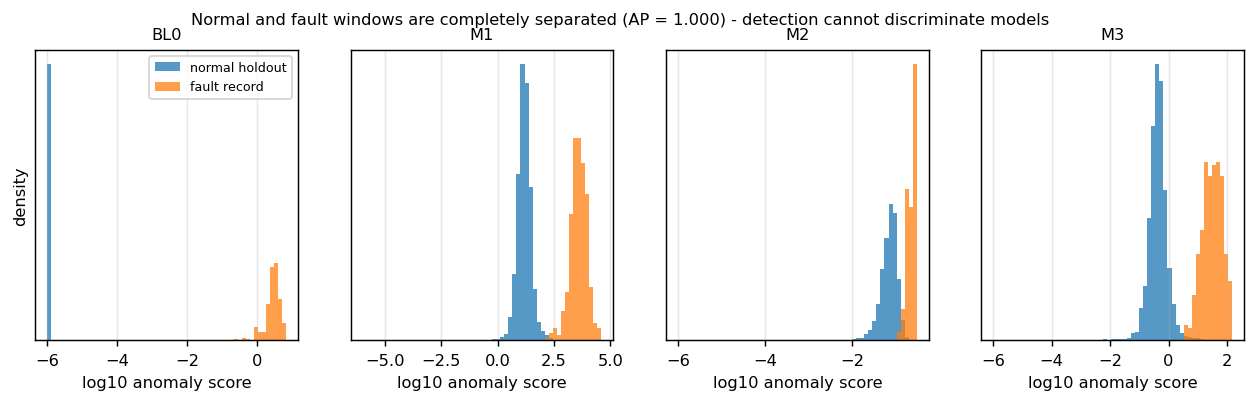
\includegraphics[width=\columnwidth]{figures/fig4_score_separation.png}
\caption{Anomaly-score distributions on fold 0. Normal hold-out and fault
windows do not overlap for any monitor, including the parameter-free range
rule BL-0. No threshold choice can distinguish these methods by detection.}
\label{fig:sep}
\end{figure}

\begin{table}[t]
\caption{Five-fold block cross-validation. Detection metrics saturate; the
models are ordered only by false alarms. FAR is per hour of acquisition on the
worst hold-out block, with Poisson 95\% upper bound. BL-1 is the reference
LSTM-Autoencoder under our protocol (\S\ref{sec:bl1}).}
\label{tab:e2}
\vskip 0.08in
\centering
\small
\setlength{\tabcolsep}{4pt}
\begin{tabular}{lrrrrr}
\toprule
 & Recall & AP & AUROC & FP rate & FAR$_{95}$ \\
 &  &  &  & (worst) & (worst) \\
\midrule
BL-0 & 1.000 & 1.000 & 1.000 & 0.0201 & 566.1 \\
M1   & 1.000 & 1.000 & 1.000 & 0.0219 & 340.7 \\
M2   & 0.932 & 0.983 & 0.997 & 0.0222 & 555.5 \\
M3   & 1.000 & 0.999 & 1.000 & 0.0227 & 362.7 \\
BL-1 & 1.000 & 1.000 & 1.000 & 0.0268 & 509.2 \\
\bottomrule
\end{tabular}
\end{table}

\paragraph{Where the separability comes from.} Ablating feature groups
(Table~\ref{tab:e4}) shows that shape features alone give
$\mathrm{AP}=0.9986$ and amplitude features alone $0.9935$, while relation and
current-level features alone give $0.69$ and $0.51$. Removing any single group
leaves AP above $0.98$: the signal is redundant across groups, which is the
signature of a global difference between the two recordings rather than a
localized fault mechanism.

\begin{table}[t]
\caption{Feature-group ablation (mean AP over folds). Any single group except
R or O nearly saturates; the discriminative signal is redundant.}
\label{tab:e4}
\vskip 0.08in
\centering
\small
\begin{tabular}{lrr}
\toprule
Feature set & M1 & M3 \\
\midrule
All (A,S,R,O) & 1.0000 & 0.9988 \\
$-$A          & 0.9997 & 0.9984 \\
$-$S          & 0.9987 & 0.9810 \\
$-$R          & 1.0000 & 1.0000 \\
$-$O          & 1.0000 & 0.9987 \\
only A        & 0.9935 & 0.9772 \\
only S        & 0.9986 & 0.9956 \\
only R        & 0.6923 & 0.6922 \\
only O        & 0.5052 & 0.5058 \\
\bottomrule
\end{tabular}
\end{table}

\paragraph{Implication for the published baseline.} Since a parameter-free
range rule reaches $F_1 = 0.973$ under this protocol, the reference
LSTM-Autoencoder's reported $F_1 = 0.748$ cannot be read as evidence about
sequence modelling. It is consistent with a protocol defect: the reference
selects its threshold by intersecting precision and recall curves on a
validation set that \emph{contains 300 fault windows}, i.e.\ it uses fault
labels to place the decision boundary of a method described as unsupervised,
and it evaluates reconstruction error at only the final timestep of each
window while training on the whole window. We revisit this in \S\ref{sec:bl1}.

\section{Robustness to Benign Measurement Shift}
\label{sec:robust}

If detection metrics cannot order the models, something else must. A
maintenance monitor's central operational failure mode is raising equipment
alarms for changes that are not equipment faults---a sensor re-seated with
reversed polarity, a gain or offset drift, a timing jitter in the acquisition
system. We test this directly: we perturb the \emph{normal} hold-out data and
measure how far the false-alarm rate rises relative to the unperturbed rate.
The fault data are perturbed as well to check that detection survives.

Table~\ref{tab:e5} reports the worst case over perturbation magnitudes. The
models that were indistinguishable in Table~\ref{tab:e2} differ by more than a
factor of five. A DC offset of half a training standard deviation drives M1's
false-alarm rate from $\approx\!2\%$ to $89.8\%$ of normal windows; the range
rule BL-0 collapses under a gain change. PCA-MSPC is the most stable, with a
worst-case increase of $17.0$ points. Meanwhile recall on fault data is
essentially unaffected for BL-0, M1 and M3 (drop $\le 2.4$ points), precisely
because recall is already saturated---confirming that the perturbation test is
informative only on the normal side.

\begin{table}[t]
\caption{Worst-case percentage-point increase in false-alarm rate when
\emph{normal} hold-out data undergo benign measurement perturbation. Lower is
better. Recall drop on fault data is shown for reference.}
\label{tab:e5}
\vskip 0.08in
\centering
\small
\setlength{\tabcolsep}{4pt}
\begin{tabular}{lrrrrr}
\toprule
 & Gain & Offset & Polarity & Jitter & Recall \\
 &  &  &  &  & drop \\
\midrule
BL-0 & \textbf{61.3} & 30.0 & 0.5 & 16.3 & 0.0 \\
M1   & 8.3 & \textbf{89.7} & 5.3 & 23.2 & 0.2 \\
M2   & 22.3 & 5.0 & 1.9 & 6.6 & 2.6 \\
M3   & 6.3 & 17.0 & 11.3 & 3.5 & 2.3 \\
\bottomrule
\end{tabular}
\end{table}

This result has a direct system-design consequence. Because a benign
measurement change can produce a large anomaly score, a single-threshold
alarm conflates two categories that demand different responses. We therefore
emit a three-level signal: \emph{green} when $p_{\text{normal}} > \alpha$;
\emph{red} when both a full-feature monitor and a second monitor restricted to
vibration-only features (excluding all current-derived features) agree, for
three consecutive windows; and \emph{yellow} otherwise---an alert whose
recommended action is to verify sensor mounting, polarity, gain and
acquisition timing before scheduling equipment inspection.

\section{Calibration and Error Structure}
\label{sec:calib}

\paragraph{Coverage.} Equation~\ref{eq:conformal} is exact under
exchangeability; overlapping windows violate it. Table~\ref{tab:e8} reports
realized coverage on normal hold-out blocks. M1, M2 and M3 track the nominal
level within $0.017$ at $\alpha = 0.10$. BL-0 does not: its realized coverage
saturates at $0.013$ regardless of $\alpha$, because every window inside the
training range receives an identical score of zero, so the $p$-value has no
resolution below the tie mass. A model whose threshold cannot be read as a
probability is unusable for alarm budgeting, irrespective of its detection
score---a point invisible in Table~\ref{tab:e2}.

\begin{table}[t]
\caption{Realized conformal coverage $\Pr(p \le \alpha)$ on normal hold-out,
averaged over folds. BL-0's score ties destroy $p$-value resolution.}
\label{tab:e8}
\vskip 0.08in
\centering
\small
\begin{tabular}{lrrr}
\toprule
$\alpha$ & 0.01 & 0.05 & 0.10 \\
\midrule
BL-0 & 0.008 & 0.012 & 0.013 \\
M1   & 0.010 & 0.047 & 0.098 \\
M2   & 0.011 & 0.065 & 0.116 \\
M3   & 0.012 & 0.052 & 0.113 \\
\bottomrule
\end{tabular}
\end{table}

\paragraph{Where false alarms occur.} Decomposing hold-out errors by operating
regime---defined by training-fold RMS terciles, never by fault data---shows
that false alarms concentrate sharply in the low-load regime: $2.30\%$ of
low-load windows versus $0.20\%$ of high-load windows, an $11.5\times$ ratio,
rising to $4.69\%$ on the worst block. Windows in the first second of a burst
also alarm more often than later windows ($1.53\%$ vs.\ $0.94\%$). False
negatives are zero in every stratum, a direct consequence of
\S\ref{sec:sep}. The actionable reading is that this monitor's errors are
dominated by under-represented normal operating states, not by missed faults,
and that additional \emph{normal} data across load conditions would improve it
more than additional fault data.

\section{Temporal Integration: Loose Rules Do Not Help}
\label{sec:mofn}

The persistence operator of Eq.~\ref{eq:mofn} is usually recommended in its
loose form: requiring $M$ hits out of $N_{\mathrm w}$ windows rather than
$N_{\mathrm w}$ consecutive ones is supposed to reduce misses, because it
tolerates quiet stretches inside a fault, without paying much in false alarms.
We measure the whole family.

\begin{table}[t]
\centering\small
\caption{Persistence rules on the normal hold-out ($2{,}929$ windows) and the
$17$ fault bursts. Candidate windows satisfy both stages at $\alpha=0.01$;
index windows never cross a burst boundary. Delay is measured from the start of
the burst.}
\label{tab:mofn}
\begin{tabular}{lccccc}
\toprule
Rule & Bursts & $R_{\mathcal{L}_1}$ & FP win. & FP ev. & Delay (med.) \\
\midrule
consecutive 1 & \textbf{16/17} & 0.963 & 35 & 23 & \SI{0.0}{\second} \\
consecutive 2 & 15/17 & 0.916 & 12 & 9 & \SI{0.1}{\second} \\
2 of 3        & 15/17 & 0.893 & 23 & 8 & \SI{0.2}{\second} \\
\textbf{consecutive 3} & 15/17 & 0.876 & \textbf{3} & \textbf{2} & \SI{0.2}{\second} \\
3 of 4        & 15/17 & 0.853 & 8  & 3 & \SI{0.3}{\second} \\
3 of 5        & 15/17 & 0.829 & 15 & 5 & \SI{0.4}{\second} \\
4 of 5        & 15/17 & 0.811 & 4  & 1 & \SI{0.4}{\second} \\
consecutive 5 & 14/17 & 0.799 & \textbf{0} & \textbf{0} & \SI{0.4}{\second} \\
\bottomrule
\end{tabular}
\end{table}

Table~\ref{tab:mofn} contradicts the recommendation. Loosening from
\emph{consecutive 3} to \emph{2 of 3} multiplies false-alarm windows by
$7.7\times$ ($3\to23$) while detecting the same $15$ of $17$ bursts; the same
holds at $N_{\mathrm w}=5$ ($0\to15$). The reason is visible in the candidate
counts: the normal hold-out contains $35$ isolated candidate windows scattered
across the record, so widening the index window mostly brings \emph{distinct}
candidates into one frame rather than bridging a genuine fault.

A second observation changes how the trade-off should be framed. With stride
\SI{0.1}{\second} the median detection delay moves only from \SI{0.0}{\second}
to \SI{0.4}{\second} across the whole family, and the maximum from
\SI{0.0}{\second} to \SI{1.5}{\second} --- negligible against the
\SI{8}{\second} burst period. \textbf{The operative trade-off here is not delay
against false alarms but misses against false alarms}, and on that axis the
pre-registered \emph{consecutive 3} sits at a defensible point: an
$11.7\times$ reduction in false alarms over \emph{consecutive 1} for the cost
of one burst.

Table~\ref{tab:mofn} is diagnostic. The rule was fixed before results were
examined and was not changed afterwards; revising it here would be the
post-selection this paper otherwise criticises (\S\ref{sec:amend}).

\section{Reproducing the Reference LSTM-Autoencoder}
\label{sec:bl1}

We reproduce the reference architecture exactly and run it in two
configurations. \textbf{G0} follows the guidebook: absolute-value
preprocessing, index-contiguous 20-sample windows with the 100-step offset,
min--max scaling fit on the first 15{,}000 normal rows, reconstruction error
taken at the final timestep only, and a threshold chosen where precision and
recall curves intersect on a validation set containing 300 fault windows.
\textbf{G1} places the same architecture inside our protocol: raw signal,
gap-aware windows, whole-window reconstruction error, and a conformal
threshold fit on normal data only.

\paragraph{On the absolute-value step.} The guidebook applies $|\cdot|$ to all
three channels. This is worth isolating because it interacts with the
preceding results. Window RMS is \emph{exactly invariant} to this transform,
since $|x|^2 = x^2$; so are mean absolute value and peak. What the transform
does destroy is sign and phase structure---precisely the information a
sequence model could exploit that a moment-based statistic cannot. Measured
over the 14{,}871 normal windows, the transform leaves RMS, mean absolute
value and peak \emph{bitwise identical} (maximum change $0.0$), while changing
window standard deviation by up to $1.19\times10^{2}$, signed mean by
$2.78\times10^{2}$, peak-to-peak by $3.04\times10^{2}$ and kurtosis by $4.88$.
The signed mean matters here: the fault record's current channel carries a
large DC offset relative to normal operation, and that offset is exactly what
$|\cdot|$ confounds with an amplitude increase. The reference pipeline thus
discards the only information that would justify the sequence model over a
moment-based monitor, before training it. Empirically the discarded structure
is not noise: the fault record is asymmetric in opposite directions on the two
vibration channels (skewness $+0.385$ on \texttt{AI0}, $-0.586$ on
\texttt{AI1}) whereas the normal record is near-symmetric on \texttt{AI0}
($+0.023$).

\paragraph{Results.} Table~\ref{tab:bl1} reports both variants against the
published values and against our selected monitor. Two things follow.

First, \textbf{G0 reproduces the published numbers}: averaged over three
seeds we obtain $F_1 = 0.743 \pm 0.029$ against the published $0.748$, with
precision, recall and false-positive rate all within seed noise. The gap
between the reference baseline and the parameter-free rule of
\S\ref{sec:sep} is therefore a property of the reference protocol, not an
artefact of our reimplementation.

Second, \textbf{the same network reaches $F_1 = 0.959$ once the protocol is
corrected}. G1 attains recall $1.000$ on every fold and AP of $1.000$ on four
of five folds ($0.999984$ on the fifth),
matching the feature-based monitors exactly. The improvement of $+0.216$ $F_1$
is attributable entirely to evaluation and preprocessing---gap-aware windows,
raw signal, whole-window reconstruction error, and a threshold fit without
fault labels---since the architecture, optimiser and training budget are
unchanged. Even so, G1 does not overtake the one-line range rule, and it
incurs the highest worst-block false-alarm rate of any model we test
($0.0268$ against $0.0201$ for that rule). Note that the two halves of
Table~\ref{tab:bl1} are not directly comparable: the published and G0 rows
come from the guidebook's single held-out split, whereas the lower rows are
five-fold means. We give both the mean and the worst block for the latter so
that the comparison is not read off a favourable fold.

We also note that under G0 early stopping never fired: all three seeds
consumed the full 800-epoch budget despite a patience of 40 on training loss,
whereas G1 stopped between 499 and 679 epochs. The reference configuration's
patience of 120 was therefore inactive.

\begin{table}[t]
\caption{Reference LSTM-Autoencoder. G0 reproduces the guidebook protocol;
G1 places the same network in ours. The published row and G0 use the
guidebook's single train/test split, so no per-block worst case exists for
them; rows below the rule are five-fold block cross-validation, reported as
mean and worst block.}
\label{tab:bl1}
\vskip 0.08in
\centering
\small
\setlength{\tabcolsep}{4pt}
\begin{tabular}{lrrrrr}
\toprule
 & \multirow{2}{*}{Prec.} & \multirow{2}{*}{Recall} & \multirow{2}{*}{$F_1$}
 & \multicolumn{2}{c}{FP rate} \\
\cmidrule(lr){5-6}
 & & & & mean & worst \\
\midrule
Published \citep{kamp2022press} & 0.664 & 0.856 & 0.748 & 0.0195 & -- \\
G0 (reproduction, 3 seeds)      & 0.667 & 0.843 & 0.743 & 0.0193 & -- \\
\midrule
G1 (our protocol, 5 folds)      & 0.922 & 1.000 & \textbf{0.959} & 0.0127 & 0.0268 \\
BL-0 (one-line rule)            & 0.949 & 1.000 & \textbf{0.973} & 0.0080 & 0.0201 \\
M3 (selected)                   & 0.928 & 1.000 & 0.962 & 0.0116 & 0.0227 \\
\bottomrule
\end{tabular}
\end{table}

\section{Cross-Validation Does Not Predict Deployment}
\label{sec:cvgap}

The protocol of \S\ref{sec:protocol} selects a model by cross-validation and
then freezes one configuration for deployment: fit on normal blocks 0--2,
conformal calibration on block 3, leaving block 4 unseen. We report what
happens next, because it was not what the cross-validation predicted.

On block 4 the frozen system raises a first-stage alarm on
$241/2929 = \mathbf{8.23\%}$ of normal windows. The five-fold cross-validation
that selected it reports, \emph{on the identical block}, a false-positive rate
of $8/2929 = \mathbf{0.27\%}$ --- a factor of $30$. Nothing about the model
differs. The fold that holds out block 4 calibrates on block 0; the frozen
configuration calibrates on block 3, which is a quiet stretch, so the quantile
it supplies is too tight for block 4. Of the 241 non-green windows, 217 fall in
original rows $16{,}000$--$19{,}000$, and $54$ of block 4's $106$ bursts raise
at least one alarm.

This is a quantified failure of the exchangeability that split-conformal
inference assumes, induced by the blocked splitting that burst structure forces
on us. Its practical consequence is that \textbf{a cross-validated false-alarm
rate is a property of the (fold, calibration block) pair, not of the system}.
With five blocks and one fault event there is no held-out budget left to
estimate the deployed rate honestly, so we report it directly instead.

\begin{table}[t]
\caption{Comparison metrics and operating metrics are different quantities.
The upper rows reuse the same 428 fault windows in every fold; the lower rows
are the frozen configuration's own held-out block plus the fault record.}
\label{tab:operational}
\vskip 0.08in
\centering
\small
\setlength{\tabcolsep}{3.5pt}
\begin{tabular}{llrrr}
\toprule
 & Prev. & Prec. & Recall & $F_1$ \\
\midrule
\multicolumn{5}{l}{\textit{Five-fold CV (model comparison)}} \\
\quad BL-0 & 0.120 & 0.949 & 1.000 & 0.973 \\
\quad M3   & 0.120 & 0.928 & 1.000 & 0.962 \\
\quad BL-1 & 0.120 & 0.922 & 1.000 & 0.959 \\
\midrule
\multicolumn{5}{l}{\textit{Frozen configuration (operating)}} \\
\quad Stage 1 only & 0.128 & 0.640 & 1.000 & 0.780 \\
\quad Two-stage (red) & 0.128 & \textbf{0.992} & 0.876 & \textbf{0.931} \\
\bottomrule
\end{tabular}
\end{table}

Table~\ref{tab:operational} separates the two. The two-stage rule cuts false
alarms from $241$ to $3$ windows (FPR $0.0823 \rightarrow 0.0010$, a factor of
$82$) at a cost of $53$ missed fault windows. Of those $53$, $33$ ($62.3\%$)
are the first two windows of a burst, which the three-consecutive-window
requirement makes structurally unreachable; the misses are a statement about
available observation length, not about the detector.

\section{Ranking Is Not Calibration}
\label{sec:prob}

The protocol exposes $\mathrm{risk} = 1 - p_{\text{normal}}$. On the frozen
evaluation set this quantity ranks almost perfectly ($\mathrm{AP} \ge 0.99$)
and is nonetheless a poor probability: its Brier score is $\mathbf{0.487}$
against $\mathbf{0.111}$ for a constant predictor at the base rate, with
log-loss $1.695$ versus $0.382$. Of normal held-out windows, $73.1\%$ receive
$\mathrm{risk} > 0.5$. This is not a defect of the estimator but of the
reading: a conformal $p$-value is uniform under the null by construction, so
$1-p$ concentrates near $1$ even for normal data. It is a rank statistic, and
reporting it as a probability is a category error.

Where a probability is genuinely needed --- deciding whether an alarm warrants
stopping production --- we report instead the posterior implied by the
two-stage operating point ($\mathrm{TPR} = 0.876$, $\mathrm{FPR} = 0.00102$)
under assumed fault prevalence:
$P(\text{fault}\mid\text{red}) = 0.896$ at $1\%$ prevalence, $0.461$ at
$0.1\%$, and $0.079$ at $0.01\%$. The gap between the first and third is the
reason we do not recommend automatic shutdown on a single alarm.

\section{Model Selection}
\label{sec:selection}

We apply gates in a fixed order and deliberately exclude detection score as a
tie-breaker: (i) numerical validity; (ii) robustness, using the normal-side
false-alarm increase of \S\ref{sec:robust} with a 20-point limit; (iii)
worst-block false-alarm rate no worse than BL-0 within tolerance; (iv) at
least one fault burst detected; (v) conformal coverage error
$\le 0.05$ at $\alpha=0.10$. Among survivors we prefer the lowest worst-block
Poisson upper bound on alarms per hour.

Only \textbf{M3 (PCA-MSPC)} passes. BL-0 fails (ii) and (v); M1 fails (ii) on
offset with $+89.7$ points; M2 fails (ii) on gain; BL-1 (G1) fails (iii) with
the highest worst-block false-alarm rate of the set ($0.0268$ against a limit
of $0.0251$). The selected system uses M3 as the first stage and a
vibration-only Mahalanobis monitor as the confirmation stage, which also
supplies per-feature contributions for root-cause text. Top-contributing
features are stable across folds (Jaccard overlap $0.87$ for M3, $0.73$ for
M1).

We flag one asymmetry. Gates (ii) and (v) were \emph{not} evaluated for BL-1:
the perturbation study requires retraining for every fold$\times$perturbation
combination, which at the measured cost of this network (a single five-fold
run takes \SI{3.6}{\hour} on CPU) exceeds our compute budget by more than an
order of magnitude. BL-1's exclusion therefore rests on a single measured
gate, and we report it as such rather than claiming it was dominated across
all criteria.

We stress that this ranking would have been invisible---and the choice would
have defaulted to the highest-$F_1$ model, BL-0---had we used detection
metrics.

\section{Amendments Made After Seeing Results}
\label{sec:amend}

Three selection gates were changed after first results. We state the
consequence first: \textbf{under the original gates the winner is BL-0, the
parameter-free range rule, not M3} (Table~\ref{tab:gates}).

(1) The robustness gate was originally defined on fault-side recall drop; with
recall saturated at $1.000$ this quantity was $0.00$--$2.57$ points for all
models and carried no information, so the normal-side false-alarm increase was
added. (2) The false-alarm gate ``no worse than BL-0'' was given a tolerance
(relative $10\%$ or absolute $0.005$); taken literally it eliminated every
model by hundredths of a percentage point and reinstated the floor baseline.
(3) The coverage gate did not exist in the original specification and was added
once BL-0's tie structure (\S\ref{sec:calib}) was observed.

\begin{table}[t]
\caption{Selection under the original and revised gates. The revision changes
the winner. We report both rather than only the second.}
\label{tab:gates}
\vskip 0.08in
\centering
\small
\setlength{\tabcolsep}{3pt}
\begin{tabular}{lrrrcc}
\toprule
 & $F_1$ & Shift & Cov.\ err & Orig. & Rev. \\
\midrule
BL-0 & \textbf{0.973} & 61.3 & \textbf{0.087} & \textbf{pass} & fail \\
M1   & 0.965 & \textbf{89.7} & 0.002 & fail & fail \\
M2   & 0.929 & 22.3 & 0.016 & fail & fail \\
M3   & 0.962 & \textbf{17.0} & 0.013 & fail & \textbf{pass} \\
BL-1 & 0.959 & n/e & n/e & fail & fail \\
\bottomrule
\end{tabular}
\end{table}

Two further disclosures. The claim that fault data are unused holds for model
fitting and threshold selection, which are enforced by test, but \emph{not} for
model selection: the burst-detection gate, the tie-breaking sort key, and our
reading of the ablation all consult fault labels. And the fault record was
inspected during exploratory work preceding this protocol, so these results are
not a fully held-out evaluation.

\section{Limitations}
\label{sec:limits}

The fault class is one continuous recording; the 428 fault windows are
overlapping fragments of a single event, so no confidence interval computed
over windows reflects uncertainty about \emph{faults}. Normal and fault were
recorded on different days (2022-07-12 and 2022-07-17), so the perfect
separability of \S\ref{sec:sep} is confounded with date, product, tooling and
sensor state; our perturbation study shows such nuisance factors are
individually sufficient to move these models a great deal, but it cannot
decompose the observed gap. No pre-failure segment exists, so lead time is not
measurable and we make no early-warning claim. Finally, at \SI{10}{\hertz} the
Nyquist limit is \SI{5}{\hertz}, far below gear-mesh and bearing fault
frequencies \citep{randall2011rolling}; we therefore avoid any
spectral-diagnostic interpretation, and note that this also removes much of
the motivation for a high-capacity temporal model.

\section{Conclusion}
\label{sec:conclusion}

A benchmark on which every method scores perfectly is not an easy benchmark;
it is an uninformative one. On the dataset studied here, detection metrics
order methods no better than chance, while robustness to benign measurement
shift separates them by a factor of five and calibration quality eliminates
the apparent winner outright. We recommend that packaged reference analyses
for industrial datasets report acquisition structure, a parameter-free
baseline, and a measurement-shift stress test alongside any headline score. In
this instance all three would have changed the conclusion.

\section*{Reproducibility Statement}

All results are produced by a single command on CPU
(\texttt{python run\_all.py --mode quick}, \SI{25}{\second}) with a fixed
seed; the deep baseline is enabled by \texttt{--mode full}. Input file
SHA-256 digests, configuration and environment are written to a run manifest.
Three invariant tests are enforced: no window may cross an acquisition gap, no
burst may be split across cross-validation blocks, and no fitted object may
observe hold-out data. Every number in this paper is emitted to a CSV file
named in the accompanying code.

\bibliographystyle{plainnat}
\bibliography{references}

\end{document}
